% Start here


\chapter{Introduction}


The aim of this document is to report the results of the evaluation of the means of description to model the requirements of SUBSET-026 concerning the on-board unit.

This evaluation task is part on work package WP7, task 1  "Primary tool Chain analyses and recommendations". According to the results of WP2, especially the OpenETCS process and the requirements on language, the aim of this task is to determine the best candidates to  produce models of the on-board units, following the OpenETCS process

This process is described in détail in D2.3 " Description of the openETCS process" and is summed up in the figure \ref{fig:main_process}.
 

 \begin{figure}
  \centering
  \fbox{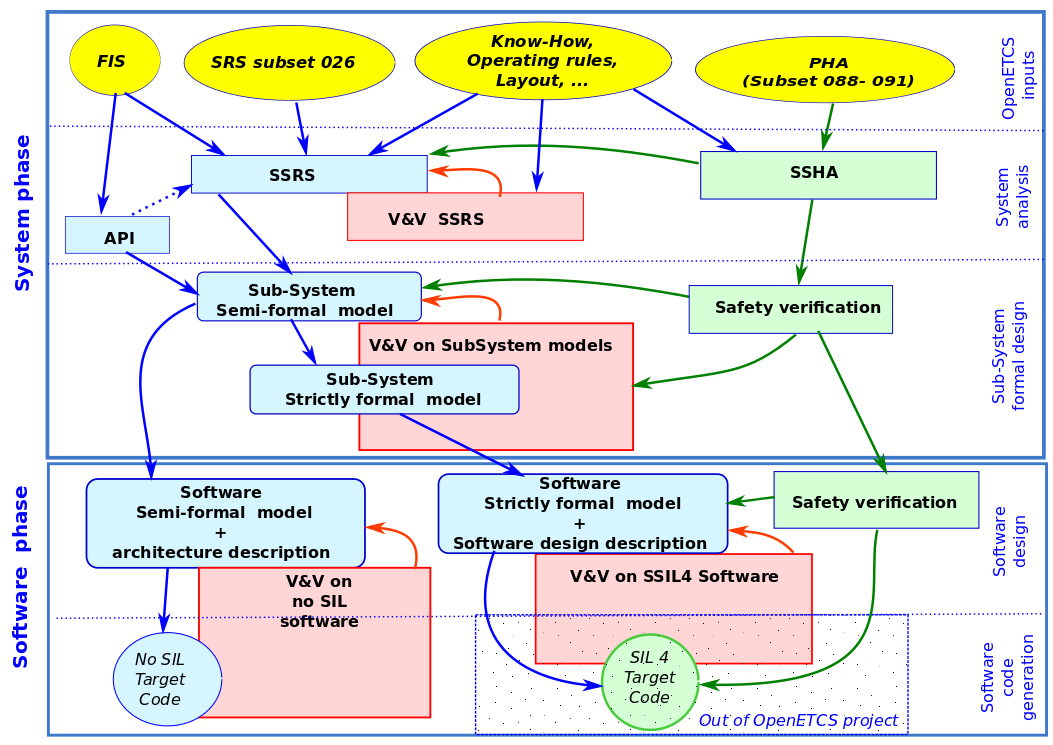
\includegraphics[scale=0.45]{WholeProcess.png}}
  \caption{Main OpenETCS process}
  \label{fig:main_process}
\end{figure}

Yellow elements are inputs, blue elements are part of the design process, red elements are verification and validation activities, green elements are safety activities. Each line (between dash or full blue lines) is a phase of the process, with a name on the right. 

The second section of this document provides a template to describe the means and a list of criteria according WP2 requirements on language and models. The objectives of this description and criteria are to allow to determine the best means of description for a given activities.

The third section resumes the results of the evaluation at the end of the benchmark activities.

In Appendix, a section is dedicated to each models produced during the benchmark activities :
\begin{itemize}
\item  CORE
\item  GOPRR
\item  ERTMSFormalSpecs
\item  SysML with Papyrus
\item  SysML with Entreprise Architect
\item  SCADE
\item  EventB 
\item  Classical B 
\item  Petri Nets
\item  System C
\item  GNATprove
\end{itemize}

For each approach, the initial  author of the evaluation is the partner in charge of the modelling. Two assessors, for each approaches,  are in charge of the review of the evaluation and can correct it or add comments.

Tools and tool platform are not covered by this document but in other outputs of WP7 : O7.1.7  "Evaluation of the tools against the WP2 requirements" and O7.1.9 "Evaluation of each tool platform against WP2 requirements, independent of target tools".
Besides, Task 7.1 is focussing on design activities : despite that some means can provide verification artefacts for example,  tools and means for validation, verification, test generation,... are in the scope of task 2 and will be analysed later.